%!TEX root = maindocument.tex

\block{Overview of the ML Model}{
	\Large
	\textbf{Origin of the Features}
\begin{itemize}
	\item Physics based, atomwise partitioned GFN2--xTB quantities are used for the features and were developed in our group and can be categorized into:
	\begin{itemize}
		\item[1.] Geomtry: e.g. Coordination Number
		\item[2.] Density: e.g. Dipole Moment
		\item[3.] Energy: e.g. Coulomb--repulsion energy
	\end{itemize}
\end{itemize}
\textbf{The Hessian Matrix}

\begin{minipage}{0.4\linewidth}
\hspace*{7pt}

\begin{itemize}
	\item The elements of the Hessian are derivatives either in respect of the coordinates of a single atom or of two atoms
	\item For the ML model, we distinguish between the diagonal blocks (blue) and off--diagonal blocks (red)
\end{itemize}
\end{minipage}%
\begin{minipage}{0.6\linewidth}
	\centering
	$\frac{\partial^2 E }{\partial r_\mathrm{A} \partial r'_\mathrm{A}}$ :~
\includegraphics[width=30pt]{Graphics/blauerBlock.pdf}~~ $\frac{\partial^2 E }{\partial r_\mathrm{A} \partial r'_\mathrm{B}}$:~
\includegraphics[width=30pt]{Graphics/roterBlock.pdf}

	
\includegraphics[width=0.7\linewidth]{Graphics/MatrixHeatmap.eps}
\end{minipage}
\hspace*{10pt}

\textbf{Connecting Features and Target}
\begin{itemize}
	\item The feature vector is either build up from the quantities of one or two atoms
	\item For ML modeling a constant feature vector length is necessary, hence two submodels are used which rely on ensemble based methods
	\item The features and targets are computed for each $3 \times 3$ block in a different orientation to achieve a consistent orientation
\end{itemize}
\begin{minipage}{0.45\linewidth}
	Model~
\includegraphics[width=30pt]{Graphics/blauerBlock.pdf}~: Here the origin is shifted to the center of two atoms and the atoms are aligned to the z--axis.
	
	\centering
	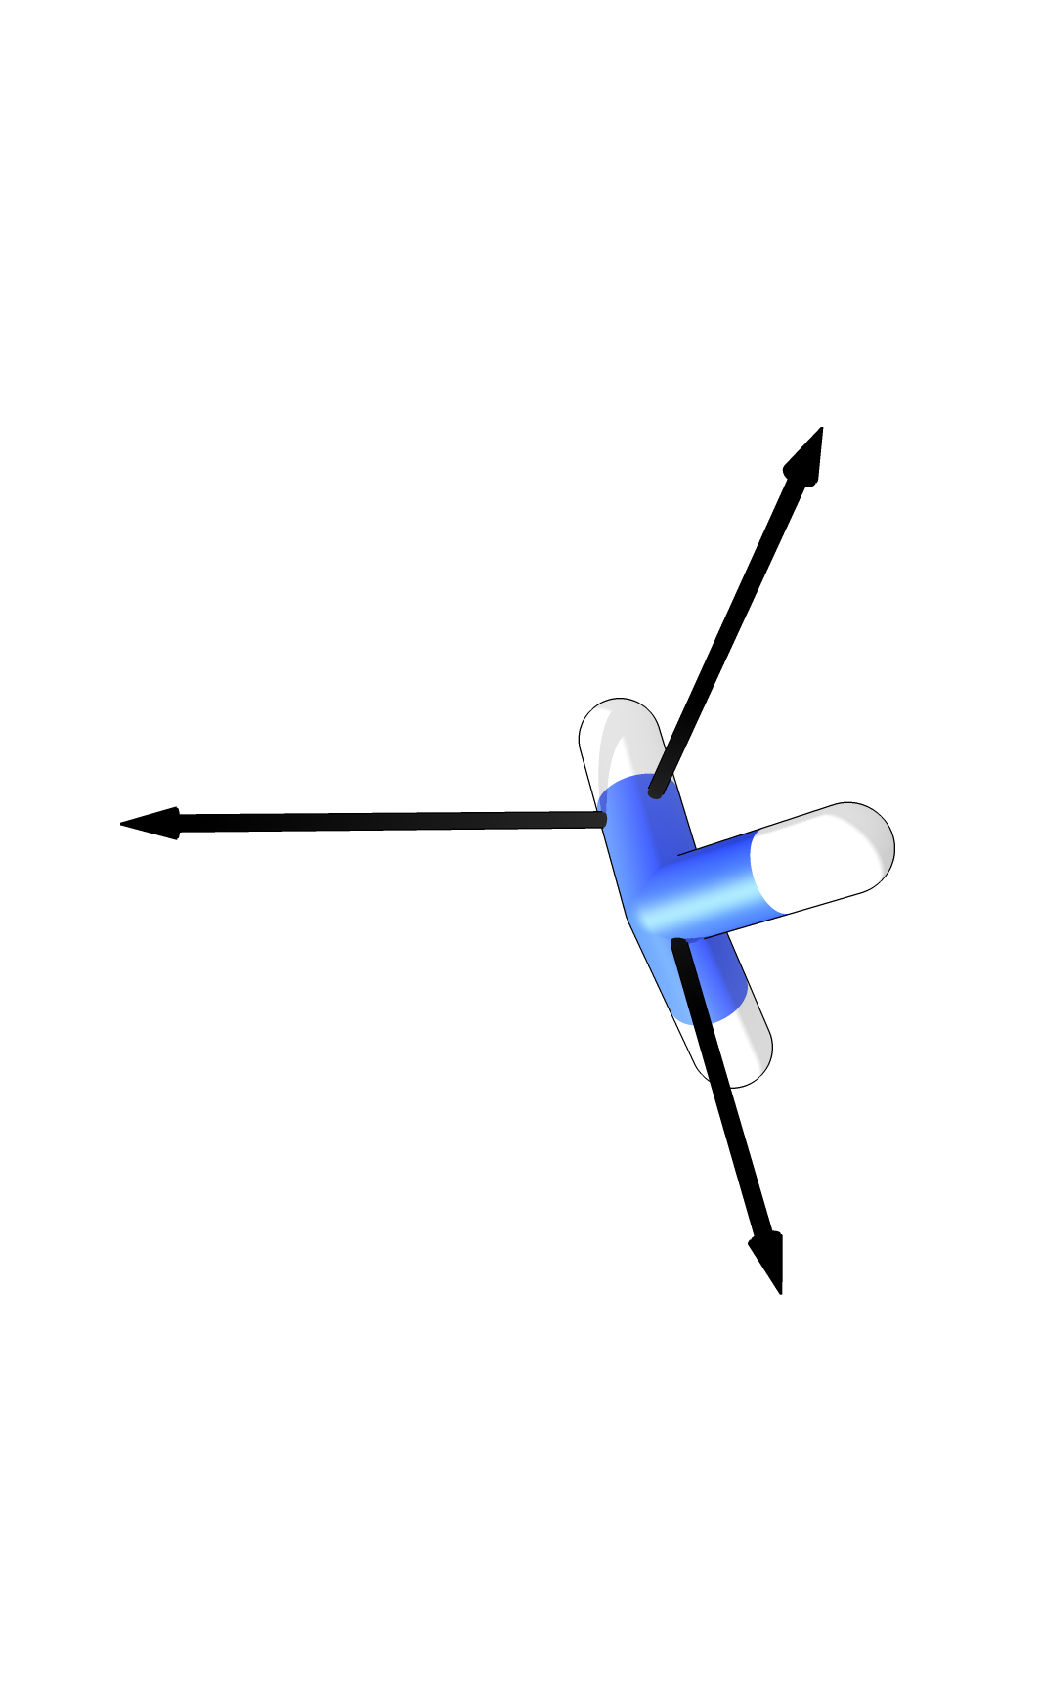
\includegraphics[angle=-90,width=0.7\linewidth]{Graphics/ndNH3.eps}
\end{minipage}%

\vspace{-14.8cm}
\hspace*{20cm}
\begin{minipage}{0.45\linewidth}
	Model~
\includegraphics[width=30pt]{Graphics/roterBlock.pdf}~: The origin of the coordinate system is shifted to the the atom.
	
	\centering
	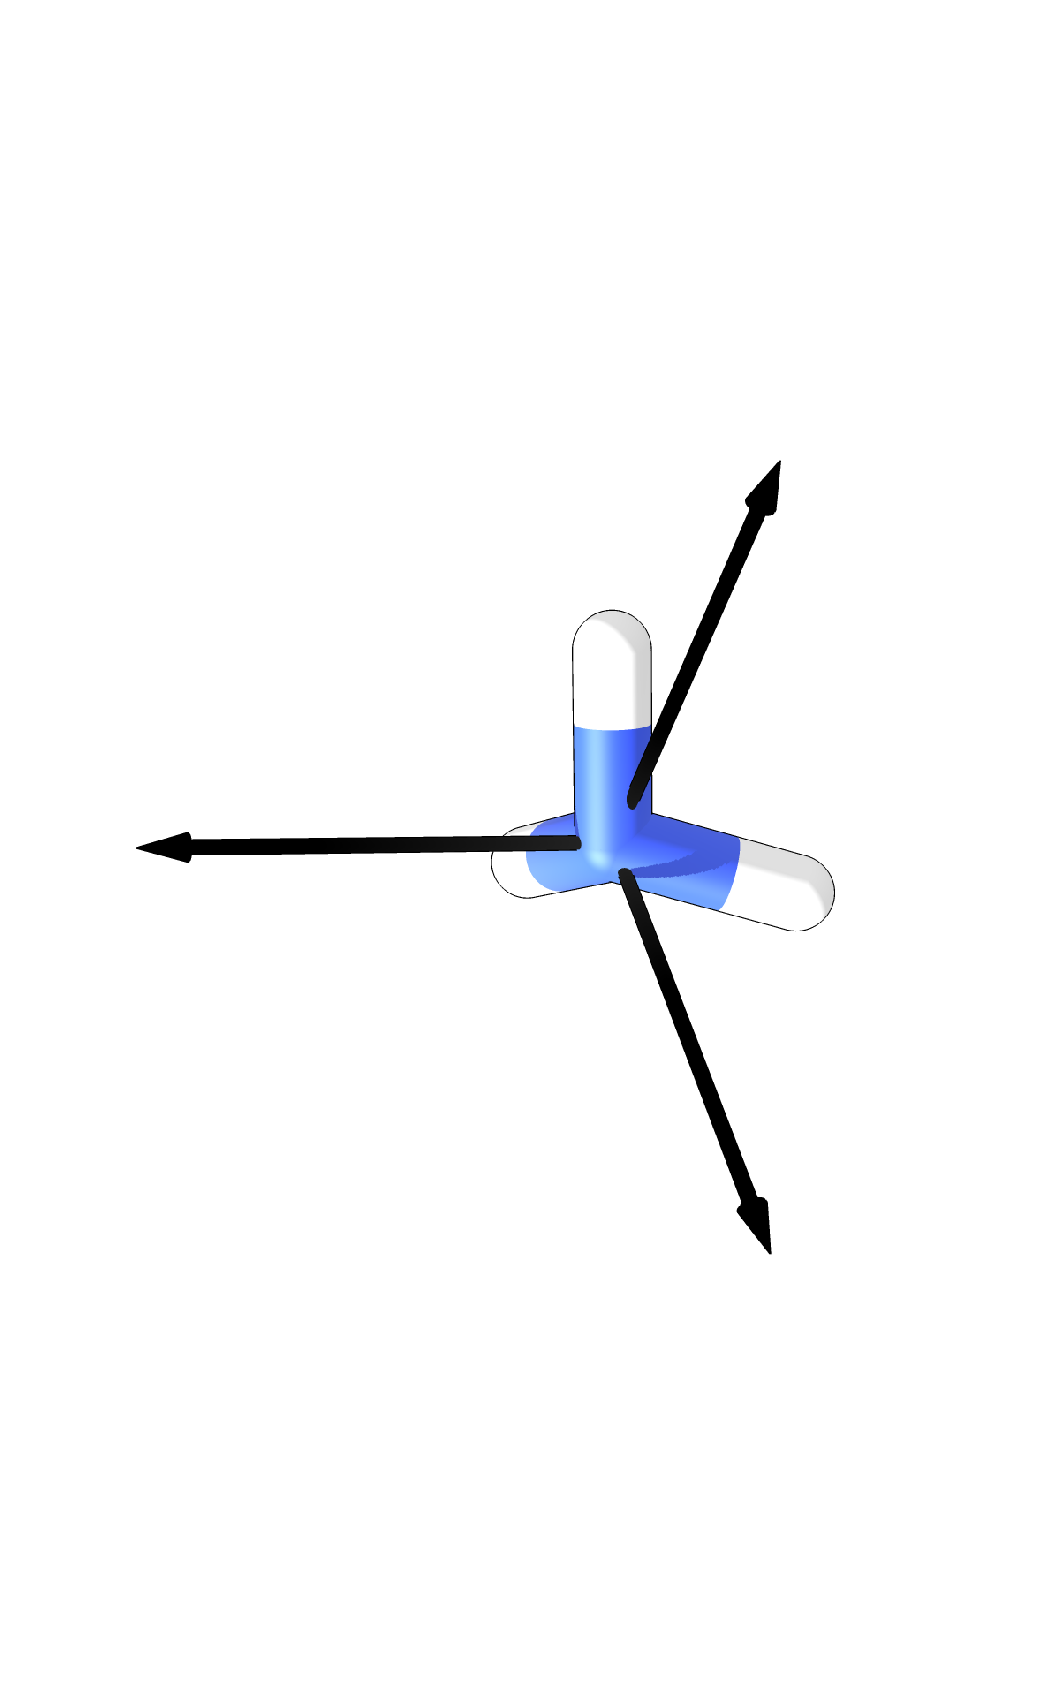
\includegraphics[angle=-90,width=0.75\linewidth]{Graphics/dNH3.eps}

\end{minipage}
\vspace*{1.5cm}

\textbf{Unifying the Mapping of the Features}
\begin{itemize}
	\item An index is introduced to differ between the the derivatives in respect to different coordinates of the same atom
	\item It is taken care of a consistent alignment to the atom oriented coordinate system
\end{itemize}
}